
\subsubsection{Input Image, \texttt{predict\_proba}}

\begin{figure}
  \subcaptionbox{Random input image of a football from the test set.\label{fig:football}}{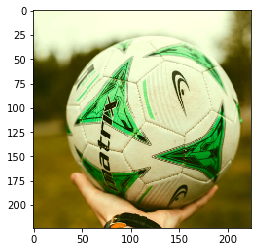
\includegraphics[width=0.49\linewidth]{../catalogue/select-35a.png}}
  \hfill
  \subcaptionbox{Random input image of tennis balls from the test set.\label{fig:tennisball}}{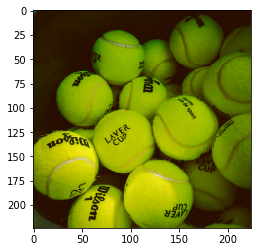
\includegraphics[width=0.49\linewidth]{../catalogue/select-35b.png}}
  \caption{Visualisation of random input images for a pre-trained image classifier.}\label{fig:balls}
\end{figure}

\begin{lstlisting}[language=Python, caption={Assertion below Figure~\ref{fig:football}. It checks if the probability estimate of the model is close to the specified value. The input image is of a football. Since the model is trained to detect tennis balls, the specified value is very small.}, label={lst:football}]
np.testing.assert_almost_equal(pred_proba, 2.0355723e-05, decimal=3)
\end{lstlisting}

\begin{lstlisting}[language=Python, caption={Assertion below Figure~\ref{fig:tennisball}. Compared to Listing~\ref{lst:football}, the specified value is much higher, since the input image contains tennis balls.}, label={lst:tennisball}]
np.testing.assert_almost_equal(pred_proba, 0.9988895, decimal=3)
\end{lstlisting}

Figure~\ref{fig:balls} presents visualisations obtained from a notebook that uses a pre-trained image classifier from the GluonCV library~\footnote{https://cv.gluon.ai}, to identify images that contain tennis balls. The visualisations are of two random input images, one from each class in the dataset. Listing~\ref{lst:football} presents the assertion related to Figure~\ref{fig:football}. The assertion checks if the probability estimate of the model for the given input image, is close to the specified value with a precision of up to three decimal places. Since the model is trained to detect tennis ball, and the input image contains a footbal, the specified probability estimate is very low. In contrast, Listing~\ref{lst:tennisball} specifies a much higher probability estimate since the input image contains tennis balls.

The above visualisation and assertion pair can be used to spot-check a few edge-cases or adversarial examples which the model may find difficult to classify. It is unclear however, how the specified thresholds were obtained since the authors do not provide additional explanation in the notebook. The threshold may have been derived based on the domain expertise of the ML practitioner. Another alternative could be to define them during the Requirements Engineering phase, by discussing with all involved stakeholders\cite{CITEME}.

In contrast to the visualisation and assertion pair in Section~\ref{sec:svm}, the assertion here is able to capture the author's motivation for visualising the input image along with the information obtained from it. Regardless, the notebook author still visualises the input image. This is a recurring phenomenon that we observe in other visualisation and assertion pairs in our catalogue. We discuss this phenomenon further in Section~\ref{sec:visual}.

\subsubsection{Normality}\label{sec:normal}

\subsubsection{Coefficient of Determination}\label{sec:r2}

\subsubsection{Normalization}

\begin{figure}
  \subcaptionbox{Histogram showing the distribution of a feature before and after scaling.\label{fig:scale}}{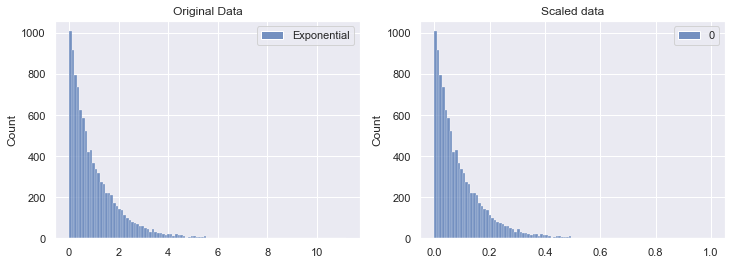
\includegraphics[width=\linewidth]{../catalogue/select-65a.png}}
  \subcaptionbox{Histogram showing the distribution of a feature before and after normalisation.\label{fig:normal}}{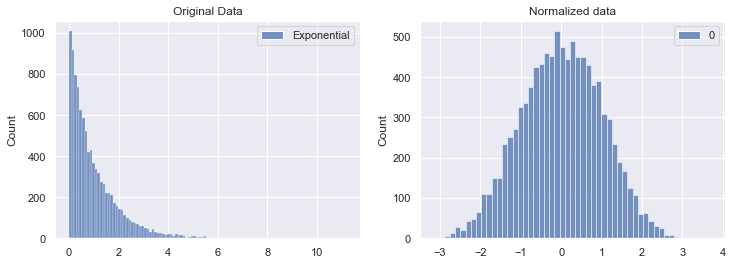
\includegraphics[width=\linewidth]{../catalogue/select-65b.png}}
  \caption{Visualisation of data before and after various data pre-processing techniques.}
  \label{fig:data-pre-process}
\end{figure}

\begin{lstlisting}[language=Python, caption={Assertion to check that the mix and max of a feature fall within specified threshold derived from the visualisation presented in Figure~\ref{fig:scale}.}, label={lst:scale}]
assert scaled_data[scaled_data.argmax()] <= 1
assert scaled_data[scaled_data.argmix()] >= 0
\end{lstlisting}

\begin{lstlisting}[language=Python, caption={Similar premise as Listing~\ref{lst:scale}, however this assertion is based on Figure~\ref{fig:normal}.}, label={lst:normal}]
assert normalized_data[normalized_data.argmax()] < 10
assert normalized_data[normalized_data.argmin()] > -7
\end{lstlisting}

Visualisations presented in Figure~\ref{fig:data-pre-process} were obtained from a notebook that presents a tutorial on scaling and normalization---two common data pre-processing techniques in ML. The visualisations show a comparison of the data before and after each pre-processing technique is applied to a feature from the data. The author scales the data using the \texttt{MinMaxScaler} from the scikit-learn library~\footnote{REFME}, between $[0, 1]$. The author performs a visual check, by comparing the distribution of the data before and after scaling, using a histogram (as shown in Figure~\ref{fig:scale}). Similarly, the author normalises the data using the \texttt{PowerTransformer} class from scikit-learn~footnote{REFME}, and performs a visual check as shown in Figure~\ref{fig:normal}.

Listing~\ref{lst:scale}~and~\ref{lst:normal} show the assertions that were defined below Figure~\ref{fig:scale}~and~\ref{fig:normal} respectively. Both assertions check that the min and max of the feature is within the expected bounds after applying the respective pre-processing technique. The assertion in Listing~\ref{lst:scale} is felt to be unneccessary since the min and max thresholds are set to the theoretical limits. The assertions in Listing~\ref{normal} are more relevant, however it is not clear why the author include such a wide margin in the thresholds.

